Дуу авианы давтамж дээр анализ хуур хөгжим хөглөдөг "Khuur" утасны аппликейшний ижил төстэй системүүдийг тайлбарлалаа. Үүнд, \emph{SoundCorset, Tunesome, ProGuitarTuner} зэрэг системүүд багтана.

\section{SoundCorset}
SoundCorset нь 30 сая хэрэглэгчтэй хөгжимчдийн аппликейшн билээ. Уг систем нь дан ганц хөглөх үйлчилгээ үзүүлэхээс гадна метроном, дуу хураагуур, рекорд хийж хөгжмийн хэмнэлийг тааруулах, дасгал сургуулалт хийхэд ашигладаг. "Khuur"-ийн хувьд зөвхөн си болон фа ноотыг л сонсож хөглөдөг бол энэ системийн хувьд бүхий л ноотыг сонсож хөглөх боломжтой. Мөн дээрээс нь нэвтрэх, дуу хураах болон хөгжмийн бэлтгэлд зориулсан тусдаа хэсэгтэй. Сул тал нь ойлгомжгүй хэрэглэгчийн интерфейс нь хэрэглэхэд болон ойлгоход төвөгтэй байна.
\clearpage
\begin{figure}[h]
	\centering
	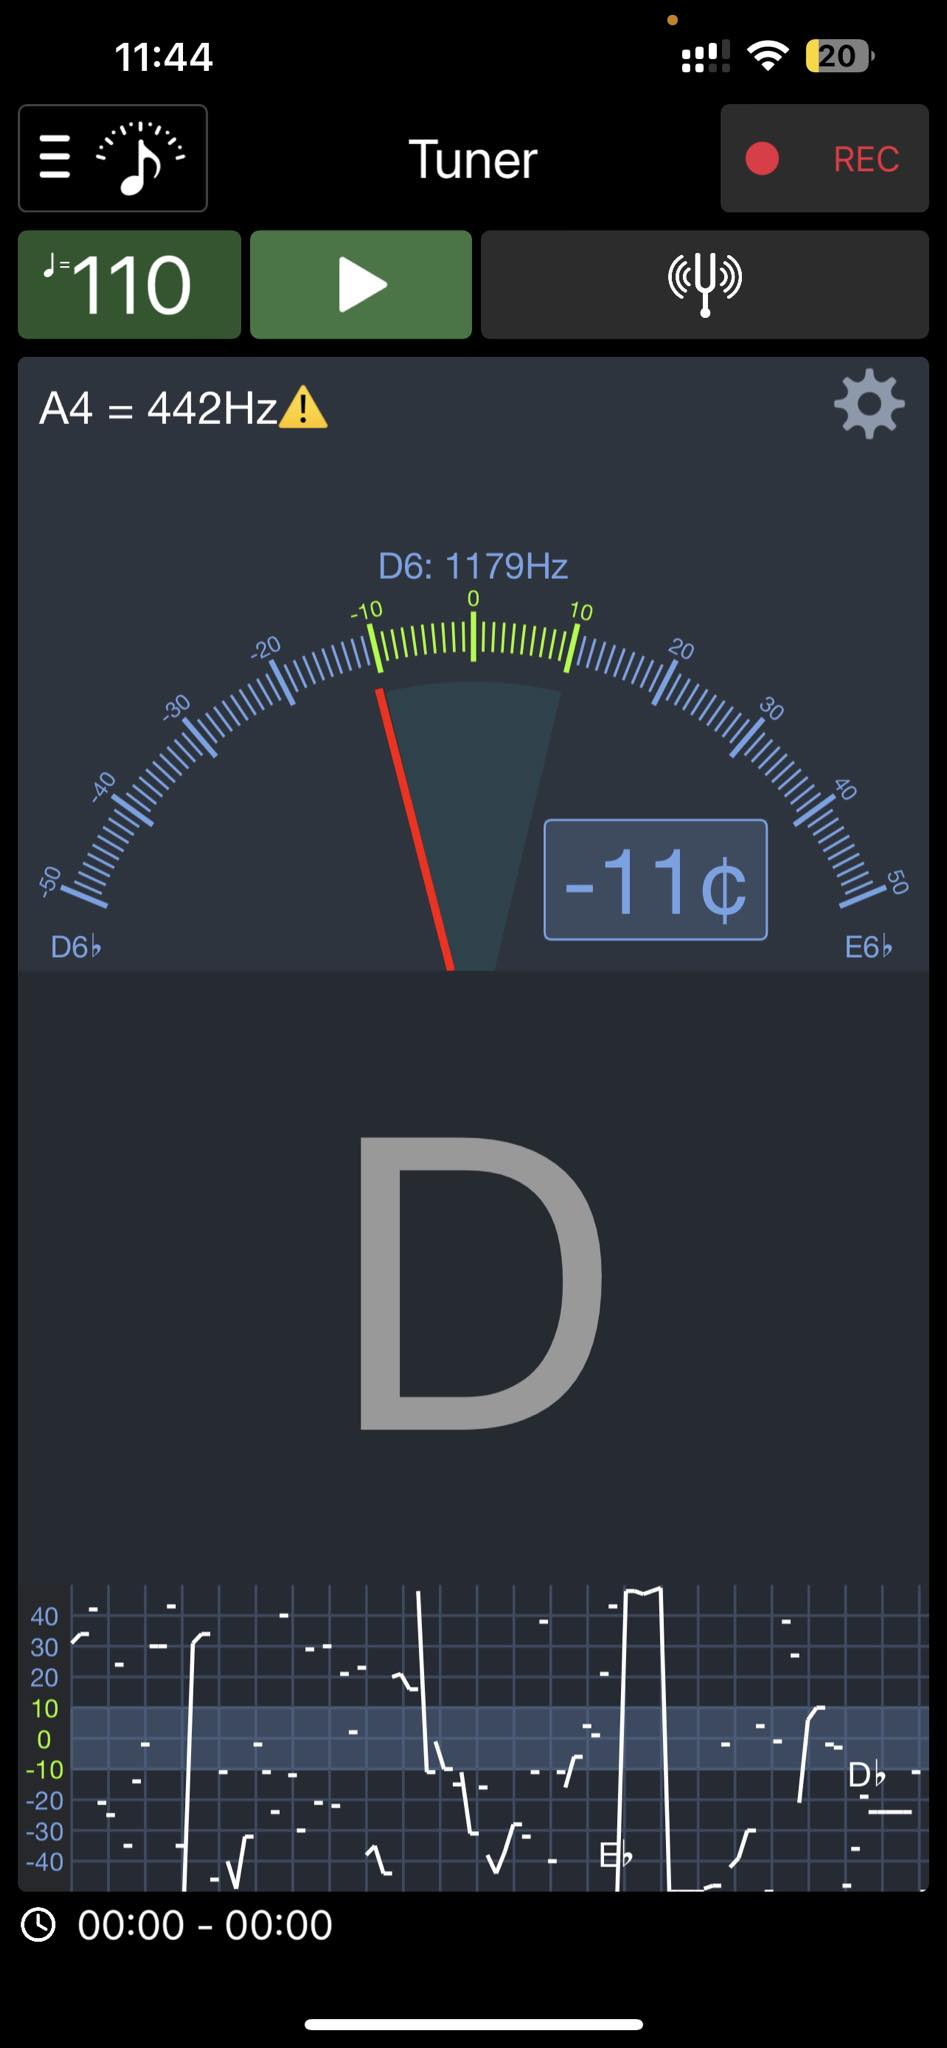
\includegraphics[height=20cm]{images/soundcorset2.jpg}
	\caption{SoundCorset-ын нүүр хуудас}
	\label{fig:modalform}
\end{figure}
\clearpage
\clearpage
\begin{figure}[h]
	\centering
	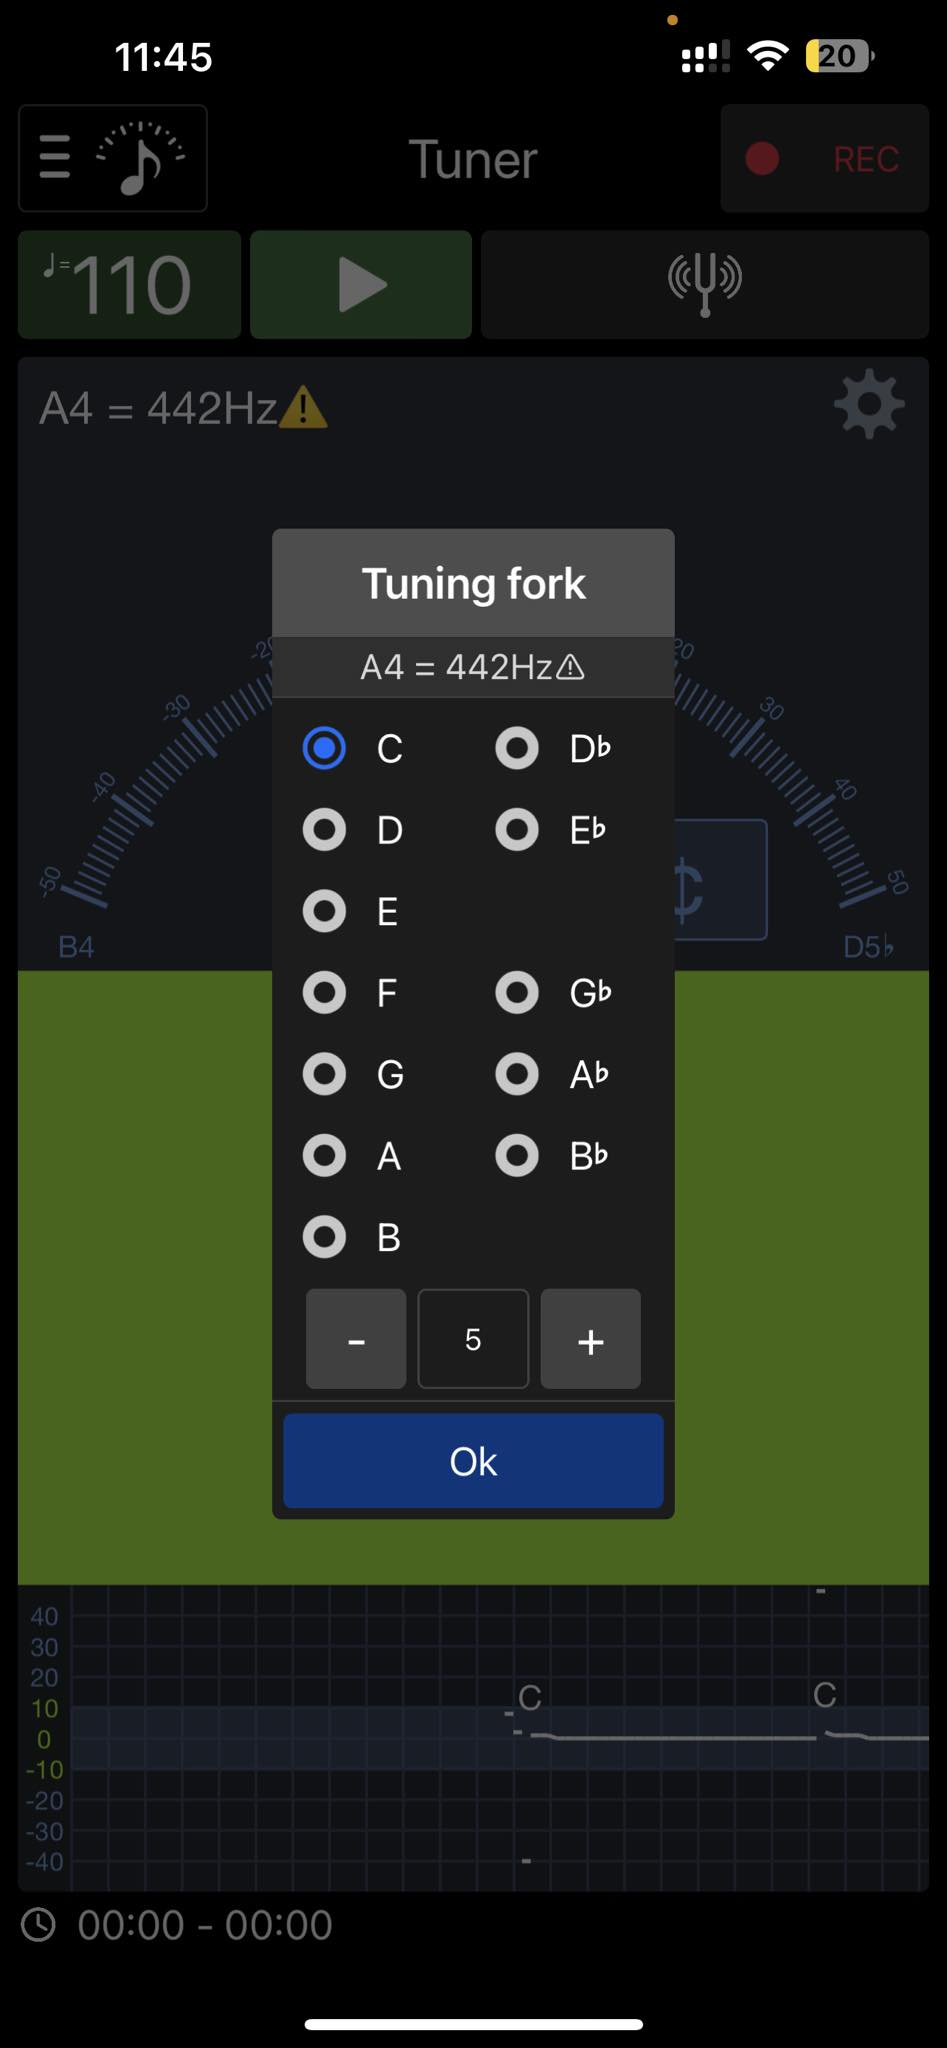
\includegraphics[height=20cm]{images/soundcorset1.jpg}
	\caption{SoundCorset-ын тохиргооны хэсэг}
	\label{fig:modalform}
\end{figure}
\clearpage
\section{TuneSome}
Tunesome бол хөгжимчдэд үнэн зөв, хэрэглэхэд хялбар хөглөх үйлчилгээг үзүүлэх зорилготой өөр нэг хөглөх аппликейшн юм. Уг систем нь мөн л олон ноотуудыг сонсож анализ хийдэг бөгөөд ихэвчлэн энгийн, хэрэглэгчдэд ээлтэй интерфейстэй нь давуу тал нь болдог. Энэхүү программ нь метроном, хөвчний номын сан, тэр ч байтугай дасгал сургуулилт зэрэг нэмэлт функцуудыг өгч, анхан шатны болон ахисан түвшний хөгжимчдийн аль алинд нь тустай хэрэгсэл болгодог. Миний сонгосон системээс интерфейсийн хувьд төстэй ч илүү хурдан, оновчтой анализ хийж байгаагаараа илүү юм. Илүү дэвшилтэт давтамжийн алгоритм ашигладаг нь ойлгомжтой байна.
\clearpage
\begin{figure}[h]
	\centering
	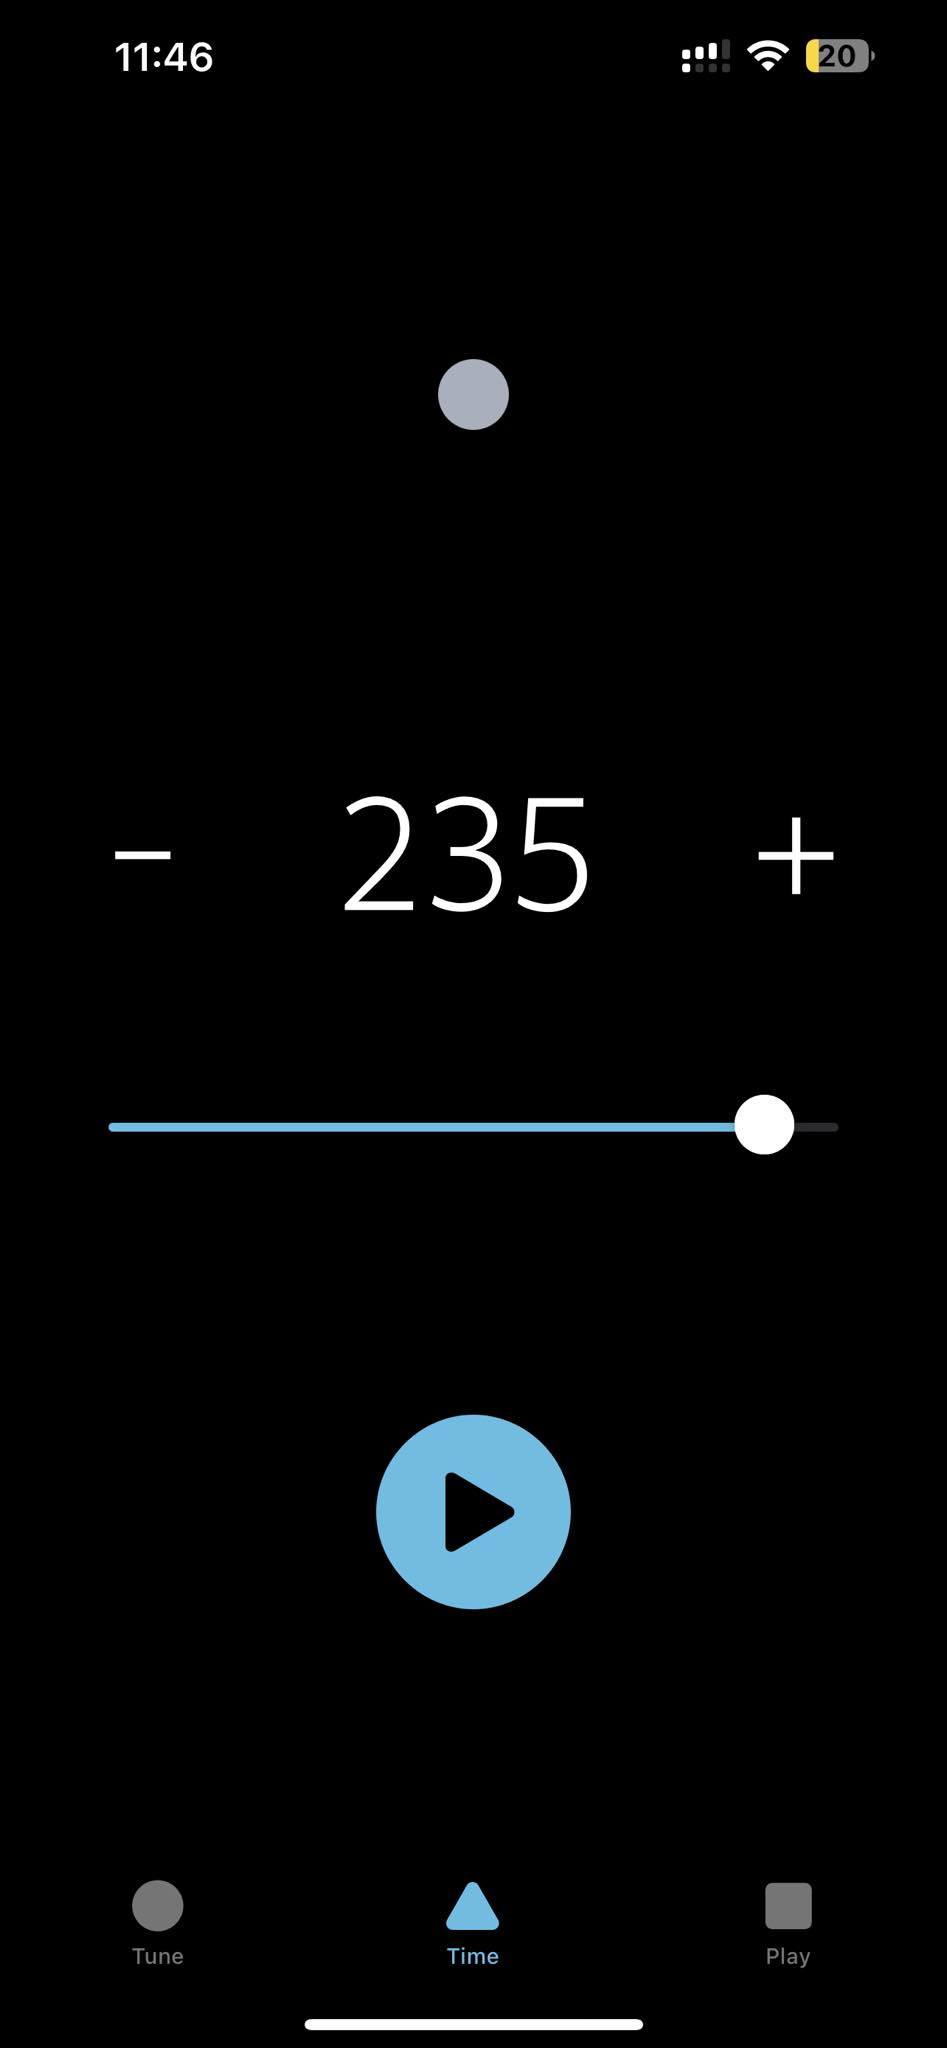
\includegraphics[height=20cm]{images/tunersome1.jpg}
	\caption{Tunesome-ын метрономын хэсэг}
	\label{fig:modalform}
\end{figure}
\clearpage
\clearpage
\begin{figure}[h]
	\centering
	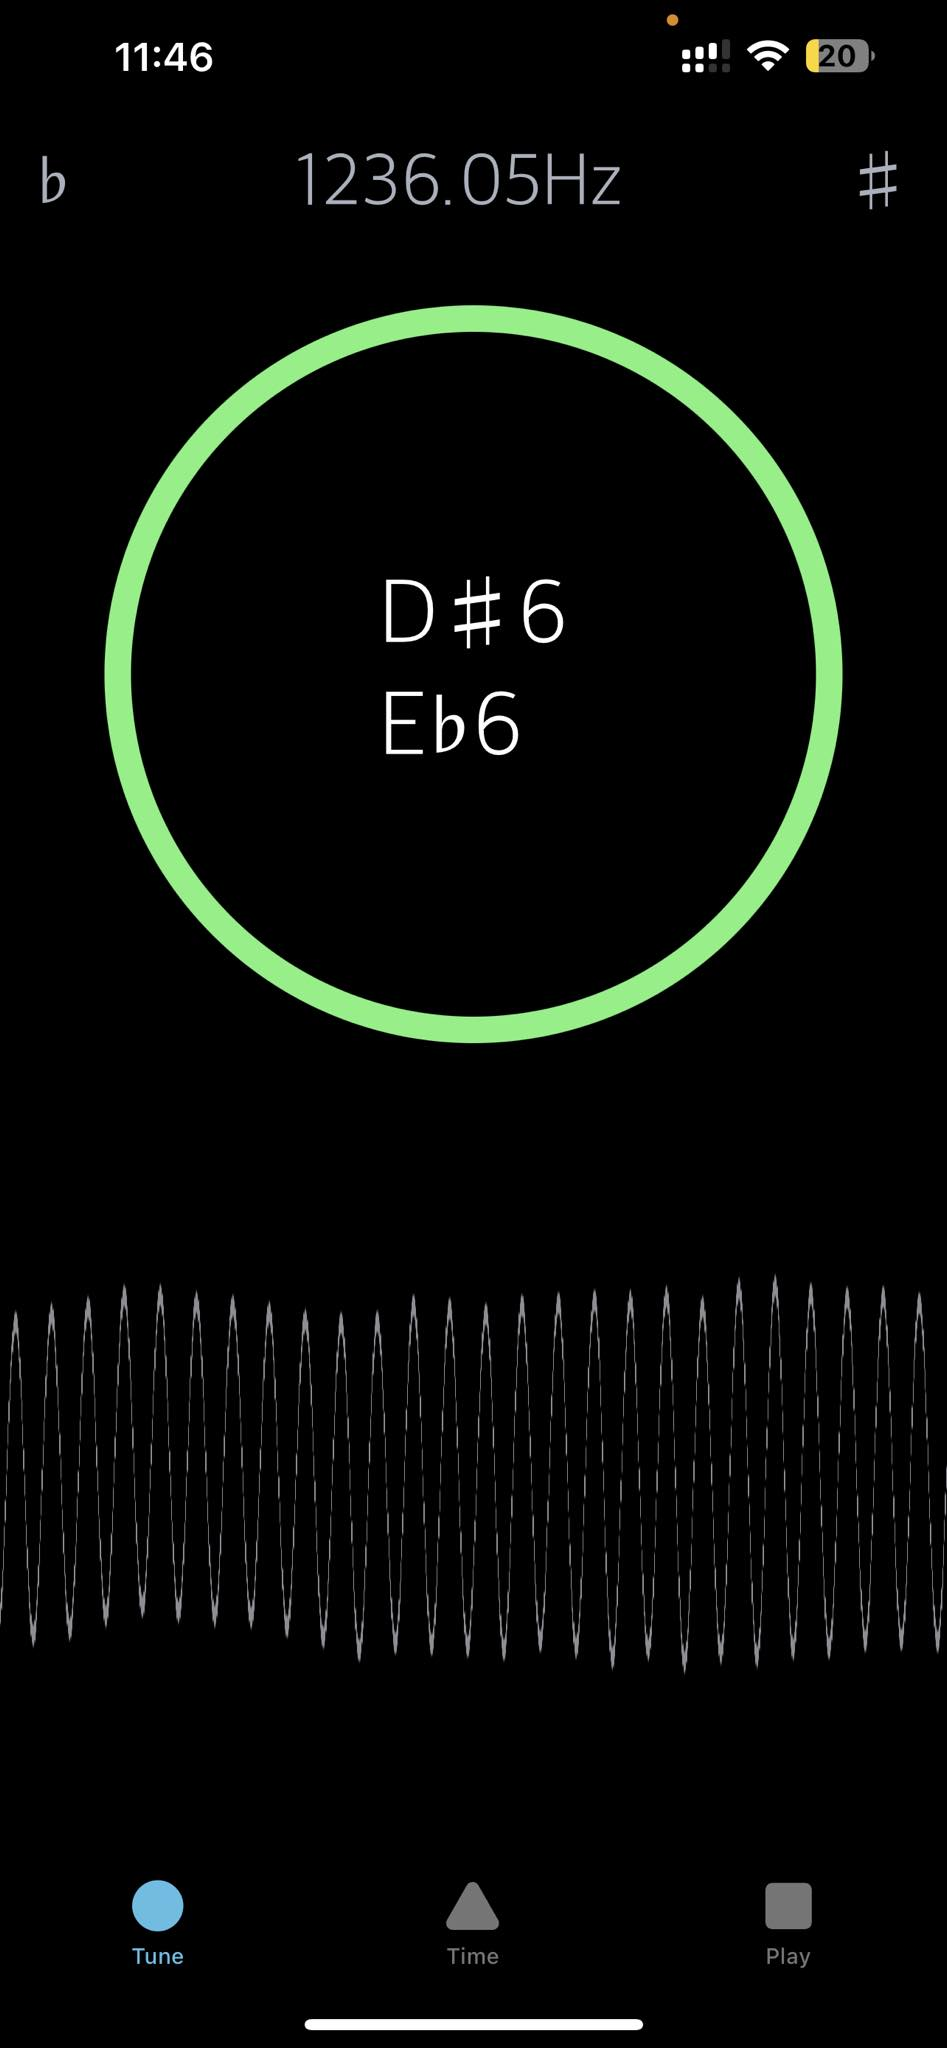
\includegraphics[height=20cm]{images/tunersome2.jpg}
	\caption{Tunesome-ын нүүр хэсэг}
	\label{fig:modalform}
\end{figure}
\clearpage
\clearpage
\begin{figure}[h]
	\centering
	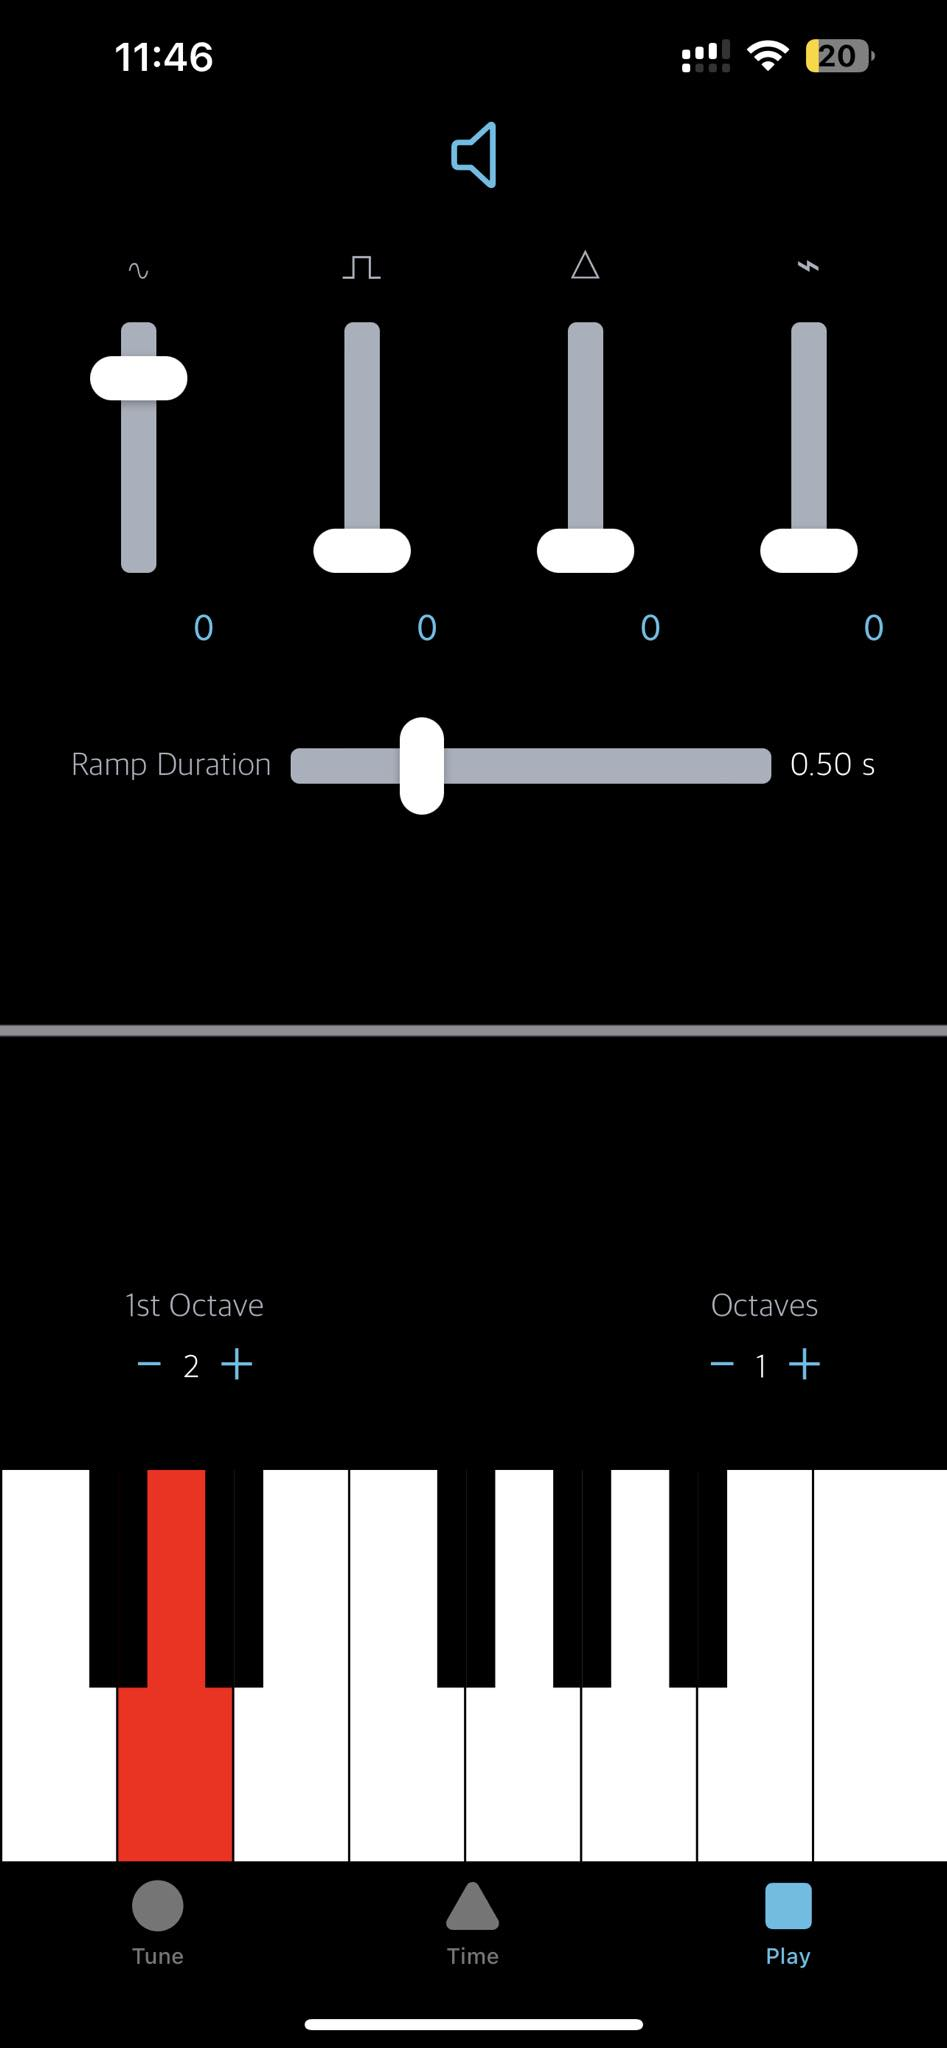
\includegraphics[height=20cm]{images/tunersome3.jpg}
	\caption{Tunesome-ын хэмнэл, давтамж тааруулах хэсэг}
	\label{fig:modalform}
\end{figure}
\clearpage
\section{ProGuitar Tuner}
ProGuitar Tuner нь гитарчдад тусгайлан зориулсан мэргэжлийн түвшний хөглөгч программ юм. Уг программ нь ихэвчлэн үнэн зөв тааруулах өндөр нарийвчлалтай алгоритмуудыг багтаасан бөгөөд давтамжийн спектрограм зэрэг нэмэлт функцуудыг санал болгодог. ProGuitar Tuner нь ерөнхийдөө гитартаа илүү нарийн мэргэжлийн, өндөр нарийвчлалтай хөглөгч хэрэгтэй хүмүүст зориулагдсан юм. Мэдээж "Кhuur"-аас ялгаатай зүйл нь морин хуур биш гитар хөглөдөг. Гэвч нэг онцлог шинж чанар нь нэг хөгжмийн зэмсэгт зориулсан шаардлагатай байж болохуйц чимхлүүрүүдийг нэмж өгсөн байна. Гитарын аль утсыг тааруулахаа хэрэглэгч сонгож болно гэсэн үг юм.
\clearpage
\begin{figure}[h]
	\centering
	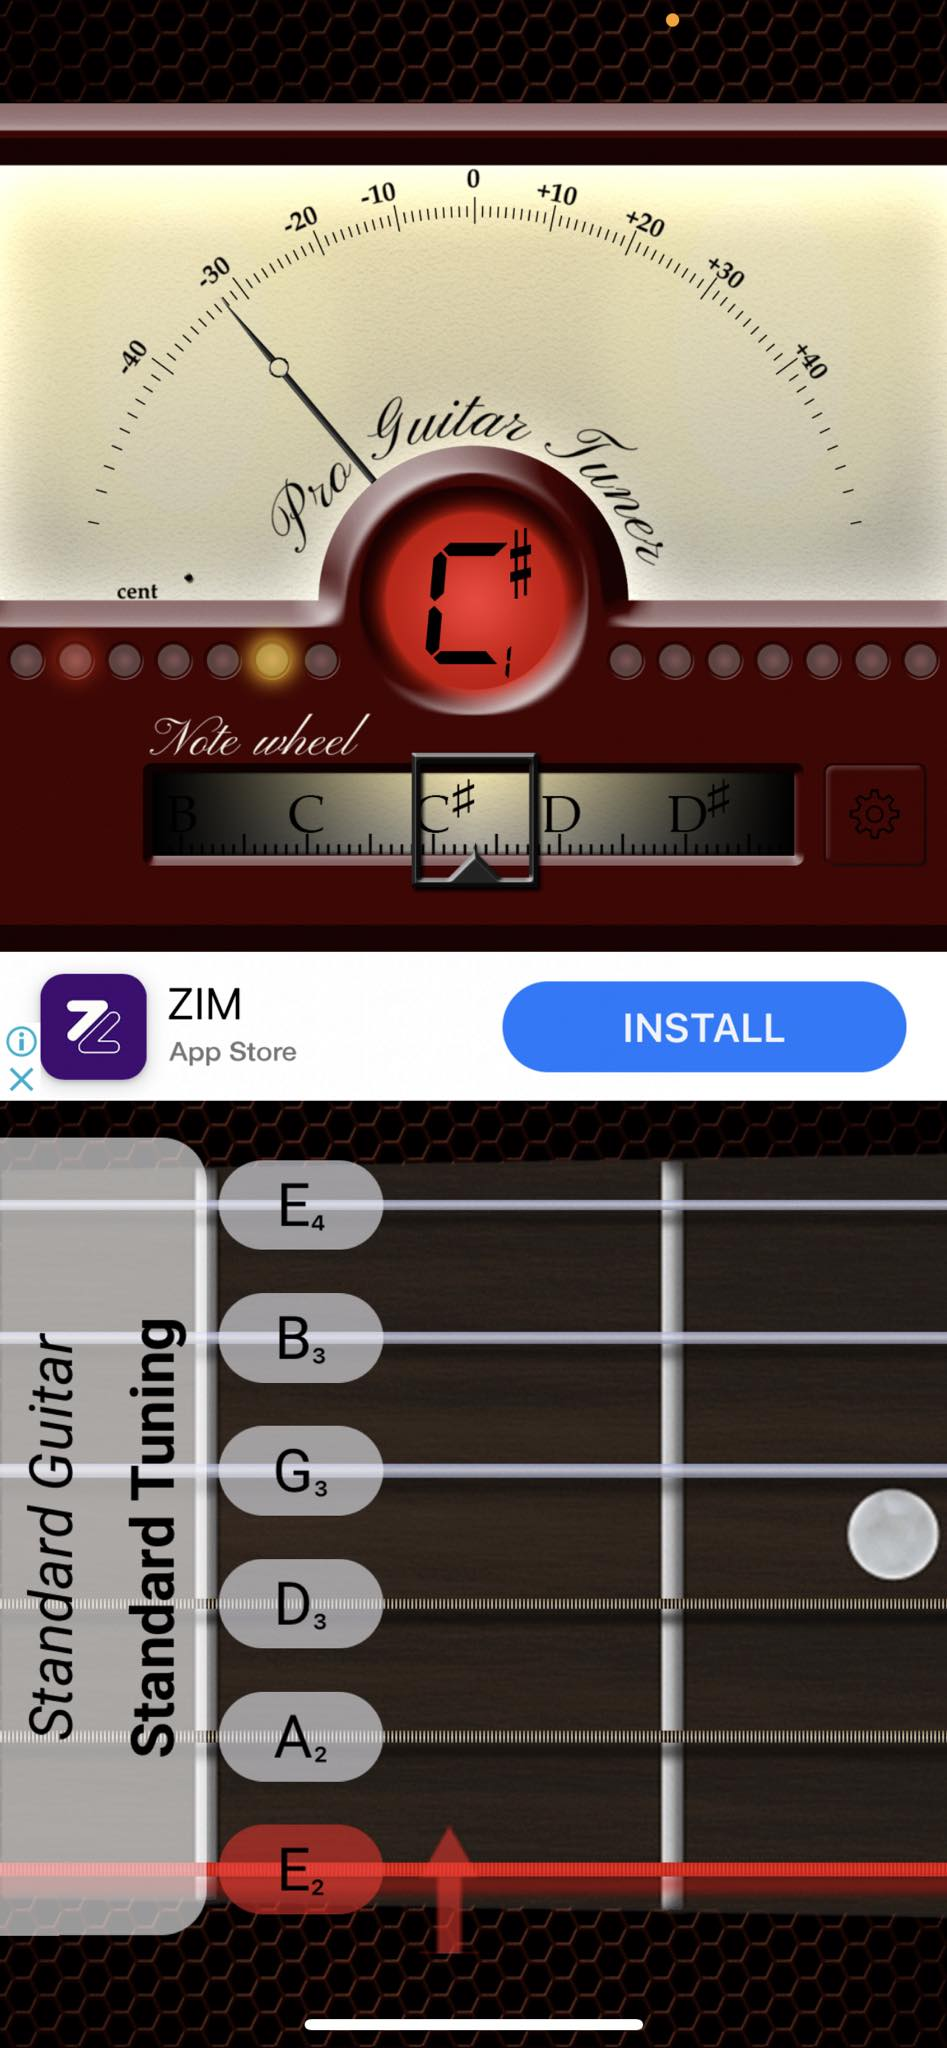
\includegraphics[height=20cm]{images/proguitartuner.jpg}
	\caption{ProGuitar Tuner-ын нүүр хэсэг}
	\label{fig:modalform}
\end{figure}
\clearpage
\section{Дүгнэлт}
Эдгээр ижил төстэй системүүдээс дүгнэхэд "Khuur" аппликейшн зөвхөн морин хуур хөглөхөд зориулагдсан учраас тэр чиглэлдээ илүү төвлөрч чимхлүүр болох нэмэлт үйлдлүүд нэмж болно. Мөн хэрэглэгчийн интерфейсийн хувьд анхлан суралцагчдад чиглэх учир аль болох минимал ойлгоход хялбар загвараар хөгжүүлэх нь чухал байна. Хэрвээ шаардлагатай гэж үзвэл яваандаа хэрэглэгчдэдээ морин хуураа давтах боломжтой шинэ үйлчилгээ нэмж болох юм.
